{\justifying
	\chapterimage{png/dataAnalysis.png}{3cm}
	\chapter{Exploratory data analysis}
	\vspace{2.5cm}
	From the data downloaded in bogota-laburbano.opendatasoft.com and library python folium was graphed the neighborhoods (Localidades) of Bogotá  with a radius of 3000 meters.
	\begin{figure}[H]
		\centering
		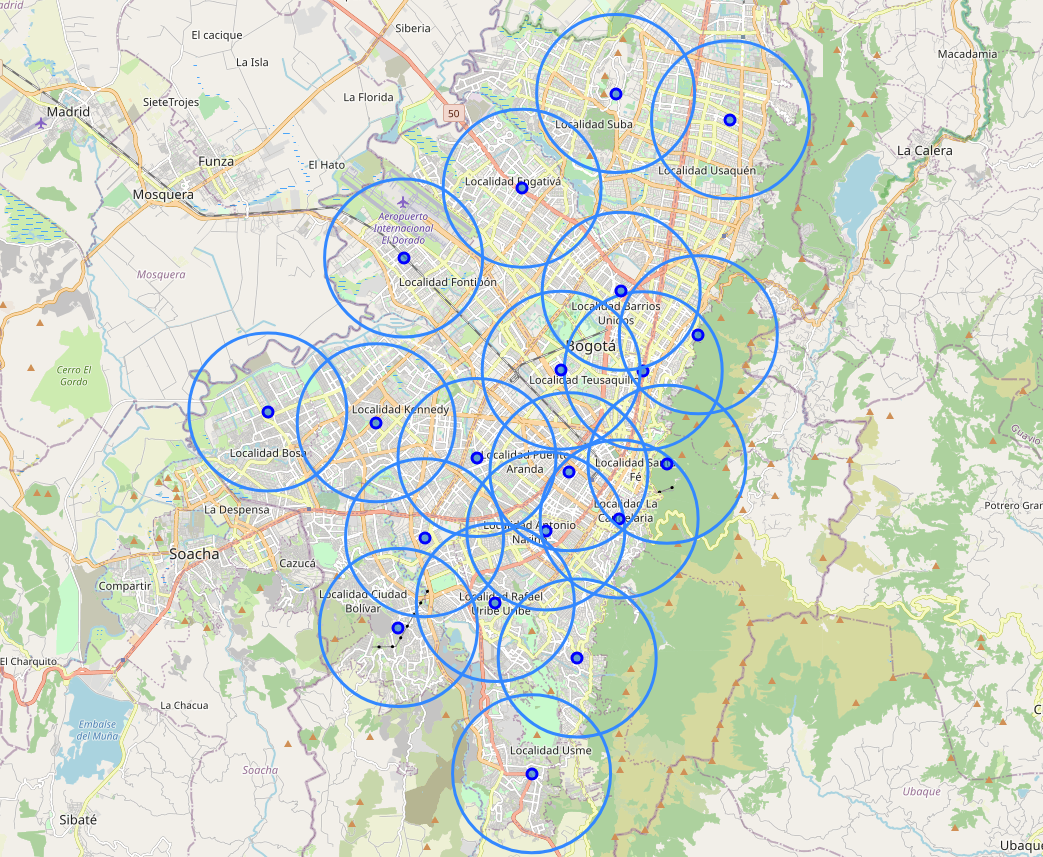
\includegraphics[scale=0.30]{png/neighborhood.png}
		\caption{Clustering}
	\end{figure}
	\section{Getting venues}
	The Foursquare API was used to find locations in each neighborhood, but, in this case, we worked with two data sets, first venues such as Restaurants (all types), GYM and Shopping Mall were analyzed because those places are important to take a decision, the other hand, the data all venues were used to analyze the similarity of the neighborhoods.
	\begin{center}
		\begin{tabular}{lll}
			\toprule
			Neighborhood &              Venue &      Venue Category \\
			\midrule
			CHAPINERO &     Bandido Bistro &   French Restaurant \\
			CHAPINERO &  Quebrada La Vieja &      Scenic Lookout \\
			CHAPINERO &    El Caracol Azul & Peruvian Restaurant \\
			CHAPINERO &       Harry Sasson &          Restaurant \\
			CHAPINERO & Brot Bakery \& Cafe &              Bakery \\
			\bottomrule
		\end{tabular}
	\end{center}
	In this way, I found the number of restaurants, GYM, Shopping Center and amount population
	\begin{figure}[H]
		\centering
		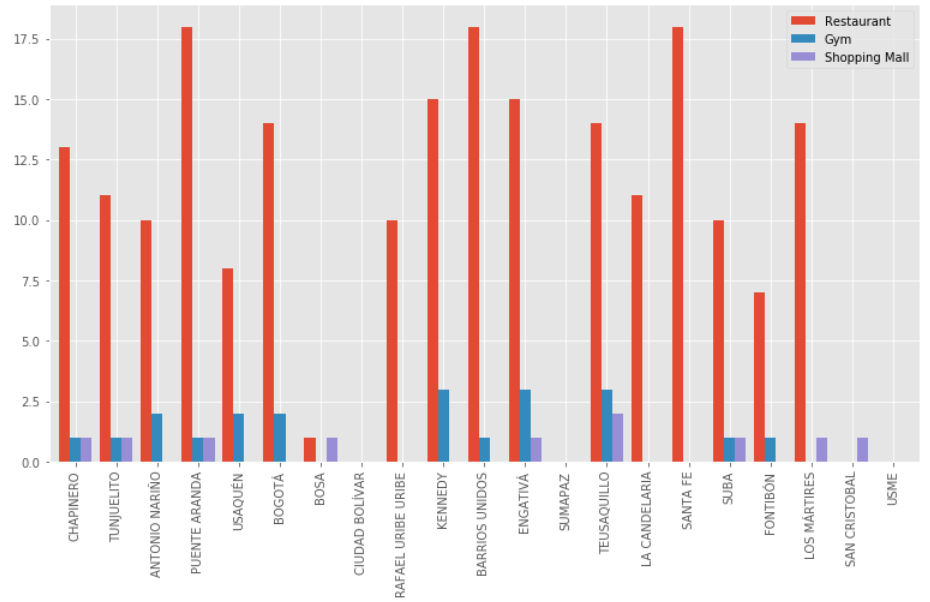
\includegraphics[scale=0.35]{png/venuesThree.png}
		\caption{Restaurants, GYM and Shopping Center}
	\end{figure}
	\begin{figure}[H]
		\centering
		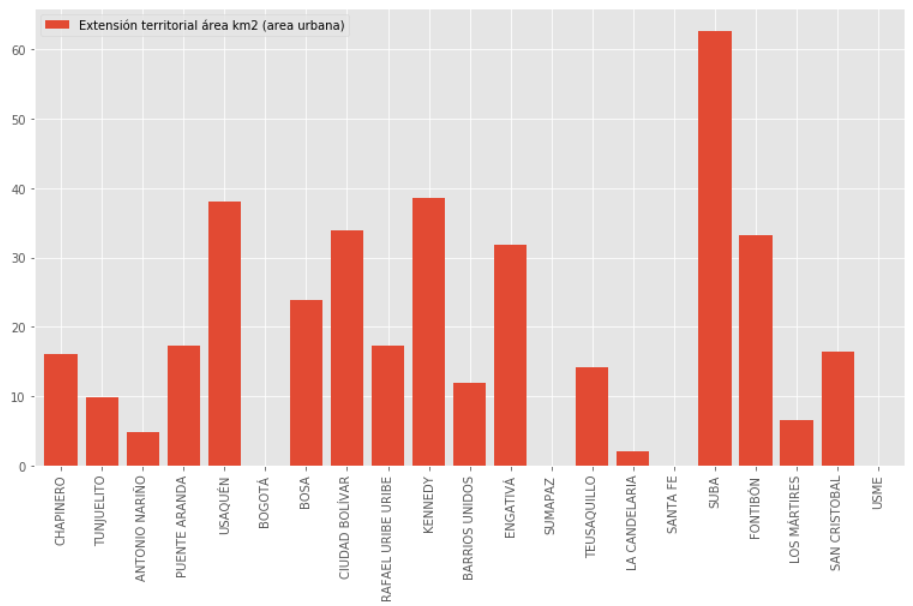
\includegraphics[scale=0.35]{png/extension.png}
		\caption{Population}
	\end{figure}
	And finally, I found the most frequent venues for each neighborhood as shown in the table
	\begin{figure}[H]
		\centering
		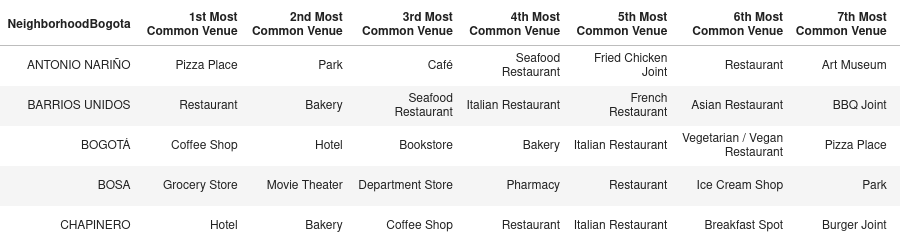
\includegraphics[scale=0.4]{png/tableVenues.png}
		\caption{The most frequent venues}
	\end{figure}
}\cleanalldata